\chapter{پیاده‌سازی و آماده‌سازی محیط استاندارد}
\section{زیرساخت پایتونی تهاجم نصف زمین}
در سال ۲۰۱۵، 
پروژه تهاجم نصف زمین \LTRfootnote{Half Field Offense (HFO)} یا همان اچ‌اف‌او
تلاش کرد محیط پایتونیی برای یادگیری تقویتی در فوتبال دو بعدی ایجاد کند.
کد سرور به گونه‌ای تغییر یافته‌بود، که بازیکن بتواند به سرور دستور اعمال رفتار‌ها و رفتن به گام بعدی را بدهد.

این روش متکی بر قابلیت‌های لیب‌سی \LTRfootnote{LibC} بود، که از آن برای ارتباط با کد \lr{cpp} استفاده می‌کرد.
لیب‌سی اجازه می‌دهد که اگر کلاس معادل پایتونی و \lr{cpp} وجود داشته باشد،
از سمت پایتون می‌توان به آن دسترسی داشت.
در این پروژه، عامل پایتونی به عنوان ایجنت دسترسی به محیط دارد، که با آن از کد \lr{cpp} محیط را درخواست می‌کند.
محیط در دو سطح بالا و پایین قابل درخواست است؛ حالت سطح پایین ۶۰ ویژگی محیط، و حالت سطح بالا ۹ ویژگی را به صورت یک آرایه صفر تا یک به عامل پس می‌دهد.
عامل سپس تصمیم خود را اخذ کرده، و به سرور دستور اجرای آن را می‌دهد.
معایب استفاده از این محیط عبارت بود از:
\begin{itemize}
    \item دشواری در تغییر محیط عامل به صورت دلخواه
    \item تفاوت زیاد بین محیط آماده‌شده در ایجنت، که مورد استفاده اکثر تیم‌هاست، و محیط اچ‌اف‌او
    \item عقب‌ماندگی محیط به علت تغییر کد‌های سرور و به روز نبودن با تغییرات شبیه‌ساز
    \item دشواری نصب، به علت پیش‌نیاز‌های قدیمی همچون \lr{Qt4}
    \item عدم امکان استفاده از تیم‌های جدید برای حریف یادگیری به علت نسخه قدیمی سرور
\end{itemize}
\section{کد پایه پایرس}
با توجه به دشواری استفاده از یادگیری ماشین در \lr{CPP}،
ما در تیم سایرس تصمیم به پیاده‌سازی یک کد پایه معادل با کد پایه \lr{Agent2D}
در پایتون گرفتیم، که نام آن پایرس \LTRfootnote{Pyrus} است.\cite{Pyrus2D}
این تلاش‌ها از سال ۲۰۱۹ آغاز شد و در نهایت بعد از سه سال و حدود ۲۵ هزار خط کد، پروژه به حالت پایدار و قابل استفاده رسیده‌است.\LTRfootnote{\url{https://github.com/Cyrus2D/Pyrus2D}}

امید بر آن بود که با توجه به اتکا بر الگوریتم‌های یادگیری ماشین به‌جای الگوریتم‌های درخت و گراف، بتوان کندی زبان پایتون را جایگزین کرد.
در کد \lr{Agent2D}،
قبل از رسیدن به گام تصمیم‌گیری، محاسبات زیادی رخ می‌دهد تا بازیکن موقعیت خود و سایر بازیکنان را بیابد، سریعترین بازیکنان به توپ، موقعیت آفساید و... را به دست آورد.
با توجه به کند بودن پایتون در مقایسه با \lr{cpp}،
همین محاسبات مقدماتی نیز بسیار زمان‌بر بودند و بخش بزرگی از ۱۰۰ میلی‌ثانیه موجود برای هر گام بازی را اشغال می‌کردند.
به همین منظور، پایرس جایگزین مناسبی برای پایتونی کردن کد نبود.

\begin{figure}[H]
    \centering
    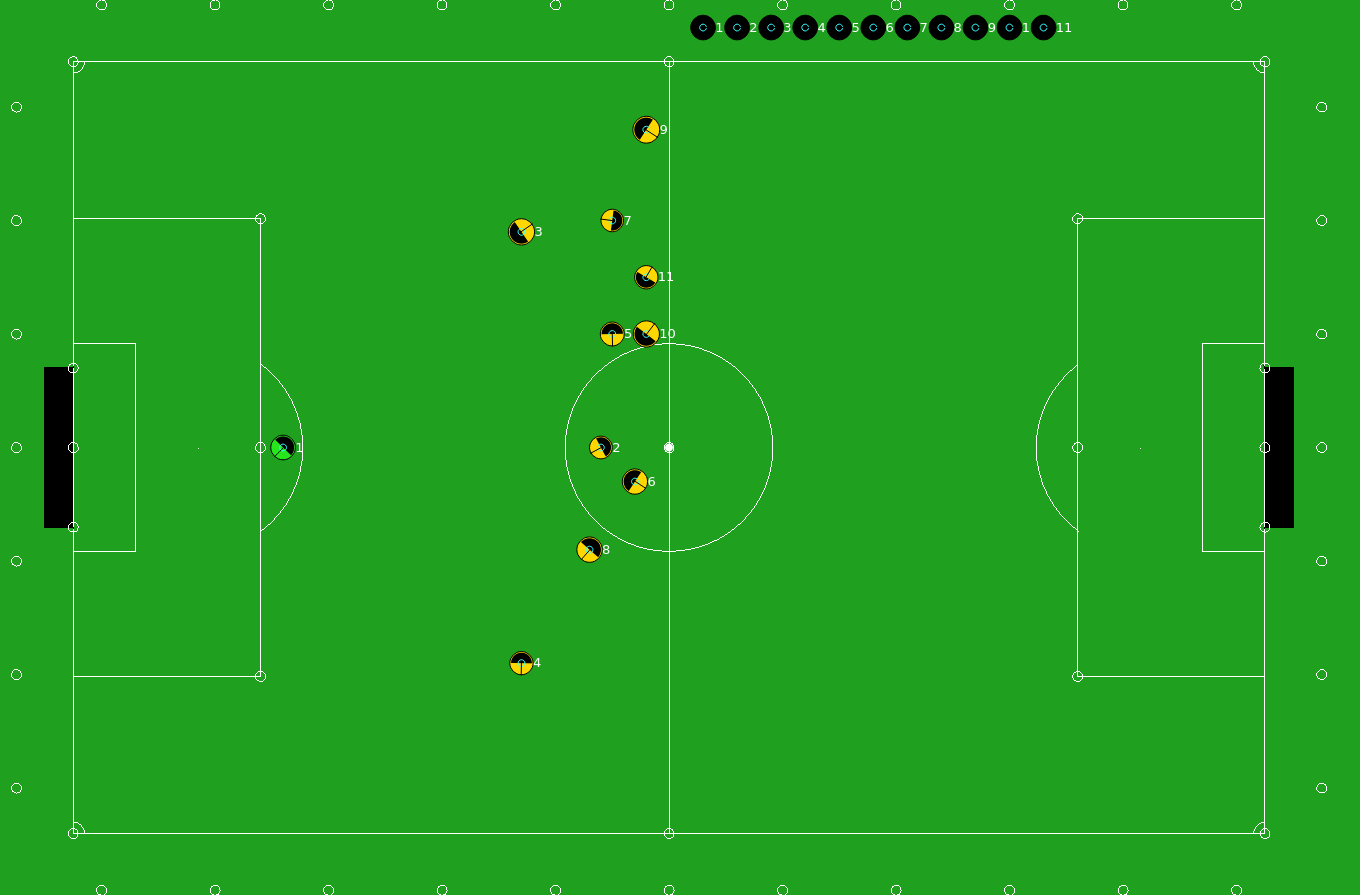
\includegraphics[width=0.75\textwidth]{images/flags.png}
    \caption{پرچم‌های کنار زمین، که برای موقعیت‌یابی استفاده می‌شوند.}\label{fig:flags}
    
\end{figure}

\section{کد پایه جی‌آر‌پی‌سی}
% TODO add grpc explanation
با توجه به سریع بودن \lr{cpp} 
برای پیش‌پردازش،
و کاربردی و راحت بودن پایتون برای یادگیری تقویتی،
تصمیم گرفتیم به کمک پروتکل فراخوانی تابع از راه دور \LTRfootnote{Remote Procedure Call (RPC)}،
این دو زبان را به هم متصل کنیم.
 در این پروژه از چارچوب فراخوانی تابع از راه دور گوگل، یا همان جی‌آر‌پی‌سی \LTRfootnote{gRPC (google Remote Procedure Call)}
 استنفاده می‌کنیم.

در این چارچوپ، ابتدا یک فایل پروتو \LTRfootnote{Proto} 
باید تعریف کرد، که حاوی مشخصات اشیاء و امضای توابع است. سپس با استفاده از کامپایلر پروتو می‌توان کد‌های سرور و کلاینت را به زبان‌های دلخواه تبدیل کرد.
سپس با اضافه کردن کد تولید‌شده توسط کامپایلر پروتو می‌توان درون کلاینت از توابع به‌گونه‌ای استفاده کرد که گویا داخل خود کد قرار دارند. از مهم‌ترین مزایای
این پروتکل ارتباطی، مستقل از زبان بودن آن، و نوشتن بسته‌های پیام به صورت صفر و یکی (در مقابل متنی)  است که سربار زمانی نوشتن و خواندن پیام را ناچیز می‌کند.
همچنین به علت استفاده از پروتکل اچ‌تی‌تی‌پی \LTRfootnote{HTTP} برای ارسال بسته‌ها روی شبکه، 
می‌توان از ضمانت‌های دریافت پیام نیز استفاده کرد.

برای تشکیل اتصال بین این دو زبان کد پایه \lr{Agent2D} را به‌گونه‌ای تغییر دادیم که
پس از اتمام مراحل پیش‌پردازش و آماده شدن مدل دنیای بازیکن\LTRfootnote{WorldModel}
در \lr{cpp}،
اطلاعات آن را با یک درخواست جی‌آرپی‌سی
به یک سرور تصمیم‌گیری پایتونی بفرستد.
در شکل \ref{fig:connection} و \ref{fig:grpc_base}
نحوه‌ی اتصال اجزای مسابقه، و روند عمومی تصمیم‌گیری نمایش داده شده‌است.

\begin{figure}[H]
    \centering
    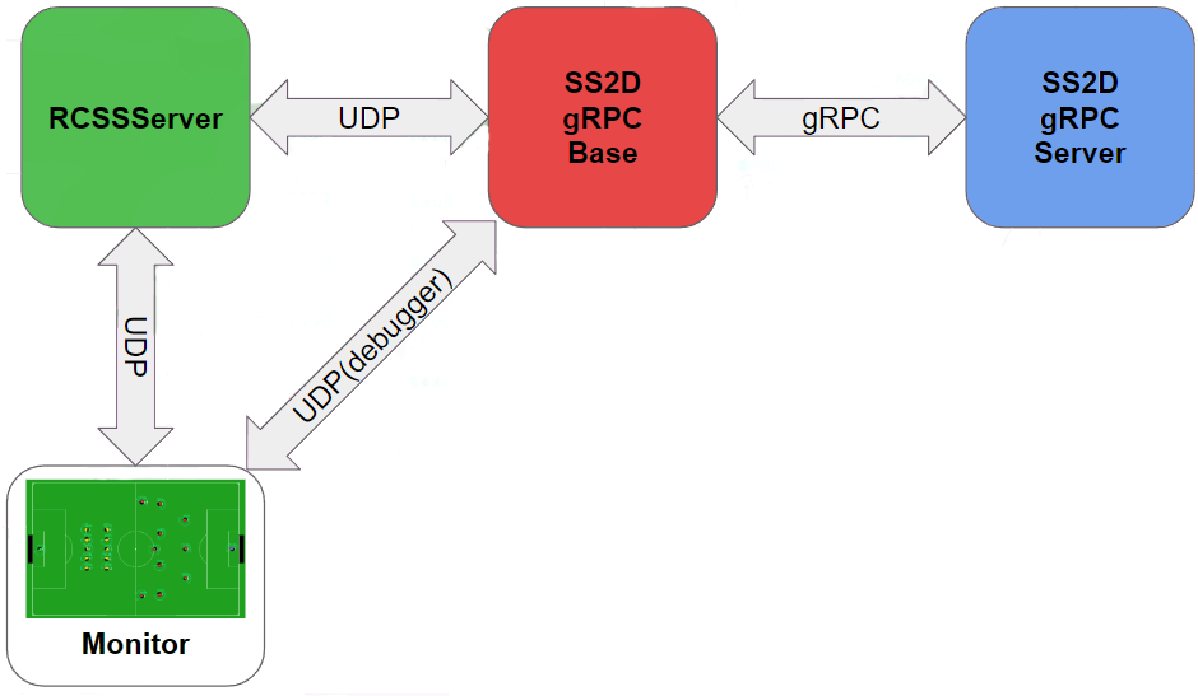
\includegraphics[width=0.75\textwidth]{images/connection_protocols.png}
    \caption{پروتکل‌های استفاده‌شده برای ارتباط بین اجزای مسابقه}\label{fig:connection}
    
\end{figure}

\begin{figure}[H]
    \centering
    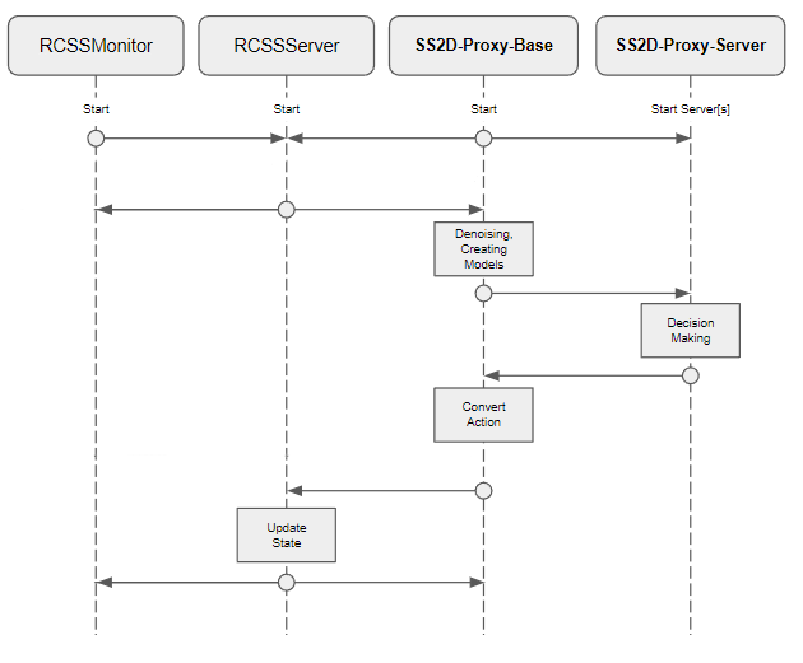
\includegraphics[width=1\textwidth]{images/grpc_base.png}
    \caption{نحوه کارکرد و اتصال کد پایه جی‌آر‌پی‌سی به سرور مسابقات و نمایشگر بازی}\label{fig:grpc_base}
    
\end{figure}
\section{محیط استاندارد جیم}
پلتفرم جیم \LTRfootnote{Gym}
که توسط گروه اپن‌ای‌ای \LTRfootnote{OpenAI}
توسعه داده شده‌است،
یک محیط استاندارد برای یادگیری تقویتی است.
این پلتفرم شامل محیط‌های گوناگون از پیش آماده شده است که می‌توانند برای یادگیری تقویتی استفاده شود.
این محیط همچنین به ما قابلیت تعریف محیط‌های جدید را می‌دهد.
\begin{figure}
    \centering
    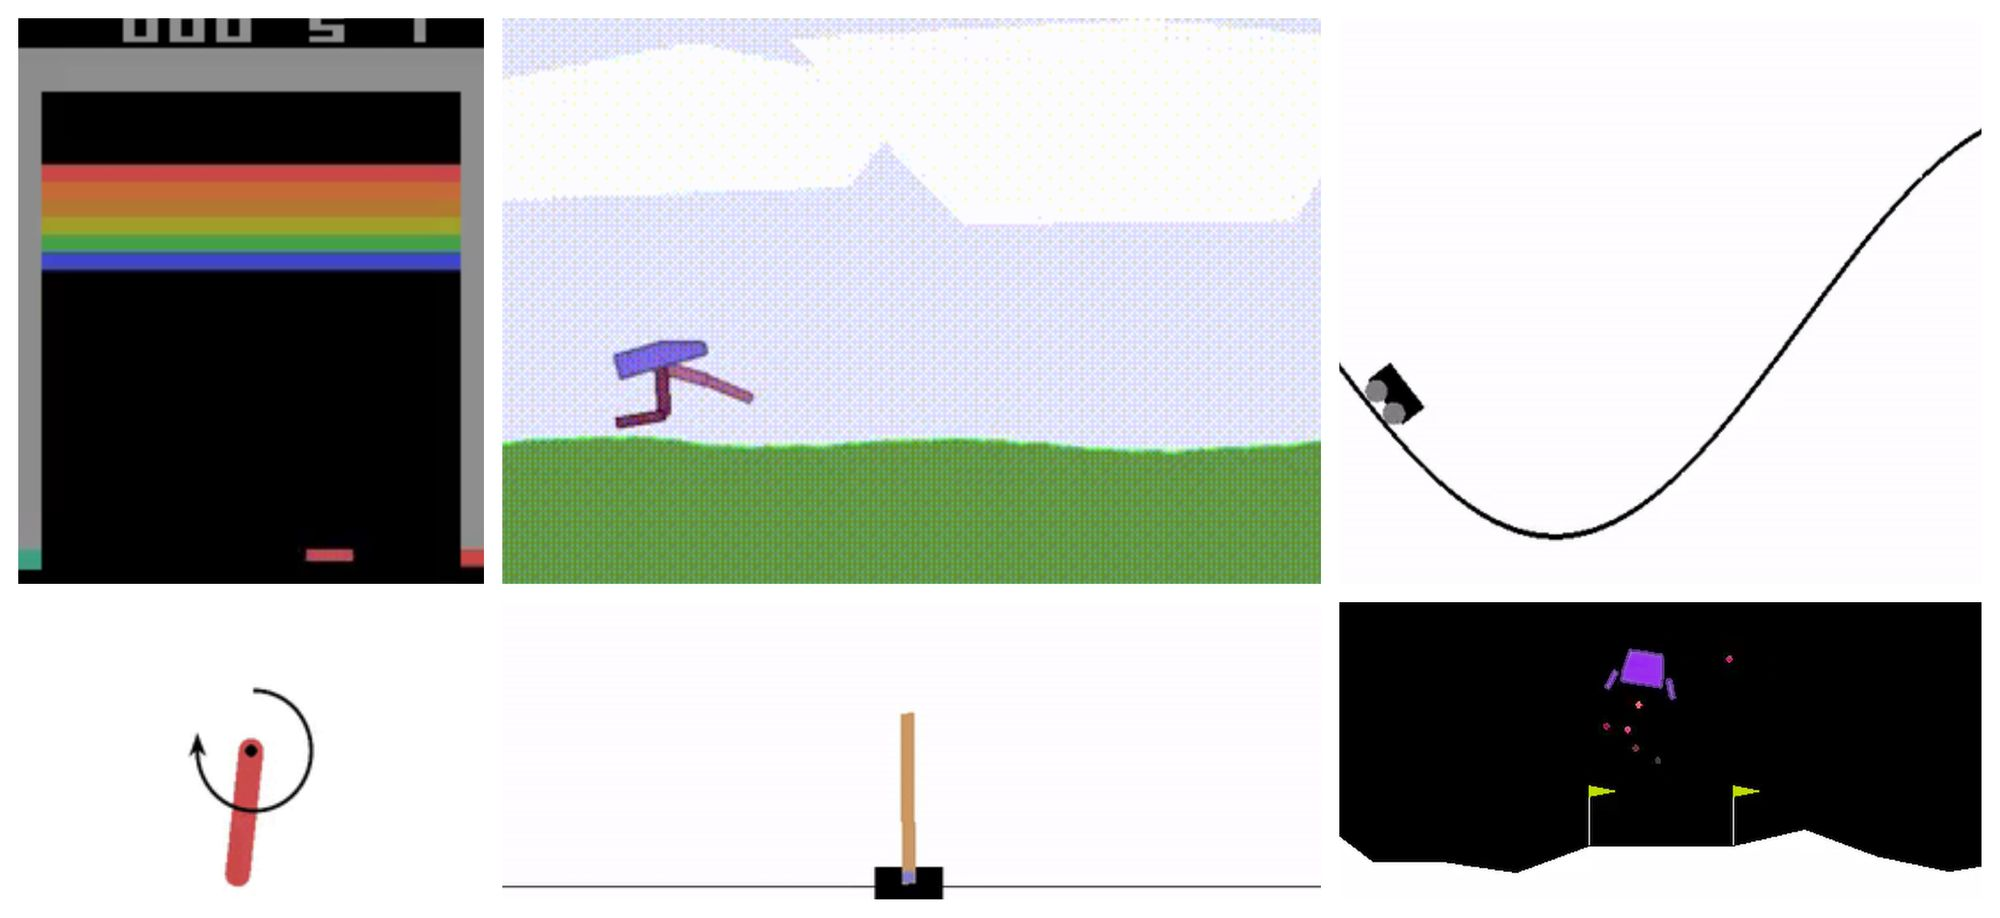
\includegraphics[width=0.75\textwidth]{images/openaigym.jpg}
    \caption{نمونه‌ای از محیط‌های آماده شده در پلتفرم جیم}\label{fig:gym}
    
\end{figure}
در سال ۲۰۲۳، 
مدیریت و نگه‌داری این پلتفرم به شرکت فاراما \LTRfootnote{Farama}
واگذار شد و از آن زمان، این پلتفرم به نام پلتفرم جیمنازیوم \LTRfootnote{Gymnasium}
 شناخته می‌شود.
تبدیل محیط یادگیری به این نوع محیط، نه تنها به ما قابلیت استفاده از کتاب‌خانه‌های پیشین و کمک گرفتن از ابزار‌های
از پیش تعبیه شده را می‌دهد، بلکه امکان به اشتراک‌گذاری راحت این محیط به سایر محققان را نیز فراهم می‌کند.
\subsection{توصیف رابط و توابع موجود}
برای تعریف یک محیط جدید در جیم،
باید توابع استاندارد آن را پیاده‌سازی کنیم. به این منظور، لازم است با روش کارکرد هر جزء محیط آشنا شویم.
لازم به ذکر است که تفاوت‌های جزئیی بین نسخه اوپن‌ای‌ای و فاراما وجود دارد، که در اینجا به توصیف نسخه فاراما می‌پردازیم.
\subsubsection{تابع گام برداشتن}
این تابع، یک عمل را به عنوان ورودی می‌گیرد،
و وضعیت جدید، پاداش این عمل، و اطلاعاتی همچون اتمام بازی، یا تمام شدن وقت عامل را به عنوان خروجی برمی‌گرداند.
\subsubsection{تابع شروع مجدد}
این تابع، محیط را به حالت اولیه باز می‌گرداند، و حالت جدید را به عامل برمی‌گرداند.
در صورتی که شروع بازی شامل المان‌های تصادفی باشد، ورودی این تابع باید کاوش تصادفی \LTRfootnote{Random Seed} را نیز به عنوان ورودی بگیرد.
\subsubsection{انواع فضا‌های حالت و عمل}
در حین تعریف محیط، باید فضا‌های حالت و عمل را نیز تعریف کنیم.
هر فضا می‌تواند از انواع زیر باشد:
\begin{itemize}
    \item گسسته \LTRfootnote{Discrete}: به ازای ورودی \lr{n}، در این فضا می‌توانیم از اعداد صحیح از ۰ تا \lr{n-1} استفاده کنیم.
    این حالت بیشتر برای فضای خروجی استفاده می‌شود.
    \item گسسته چند‌تایی \LTRfootnote{MultiDiscrete}: این فضا مشابه فضای گسسته است، با این تفاوت که می‌توانیم چند عدد از این فضا را به عنوان خروجی بگیریم.
    مشابه با گسسته است، ولی جای ورودی یک عدد، یک آرایه از اعداد است؛ هر عدد نشان‌دهنده تعداد حالت‌های ممکن در هر بعد است.
    \item فضای بسته \LTRfootnote{Box}: نشان‌دهنده یک فضای چند‌بعدی پیوسته است، که باید حد پایین و بالای هر بعد را مشخص کنیم.
    \item دوتایی چند‌بعدی \LTRfootnote{MultiBinary}: حالت چند‌بعدی است، که هر بعد مقدار صفر یا یک می‌تواند به‌خود بگیرد.
\end{itemize}
به کمک فضا‌های فوق، می‌توان فضا‌هایی از ترکیب حالت‌های فوق تعریف کرد، که به انواع زیر است:
\begin{itemize}
    \item دیکشنری \LTRfootnote{Dict}: یک دیکشنری پایتونی از فضا‌های مختلف است.
    \item چندتایی (توپل) \LTRfootnote{Tuple}: یک چندتایی مرتب از فضا‌های مختلف است.
    \item دنباله \LTRfootnote{Sequence}: یک دنباله از فضا‌های مختلف است.
\end{itemize}

\subsubsection{تابع پایان}
در اتمام کار با محیط، این تابع فراخوانی می‌شود تا محیط بسته شود، و منابع آن آزاد شوند.
\subsubsection{تابع ترسیم}
با توجه به اینکه اکثر محیط‌های جیم، به کمک کتاب‌خانه‌هایی مانند \lr{PyGame}
ترسیم می‌شوند، این تابع برای ترسیم محیط در هر گام استفاده می‌شود.
همچنین به عنوان ورودی این تابع می‌توان معین کرد که ترسیم به چه گونه‌ای انجام شود، چرا که ممکن است در حین آموزش برای تسریع عملیات، نیازی به ترسیم نباشد.
از آن‌جا که در محیط ما، وظیفه ترسیم با نمایش‌گر خارجی انجام می‌شود، این تابع برای ما معنی ندارد. 
\subsection{نحوه ادقام با فضای ربوکاپ}
برای پیاده‌سازی محیط جیم در فضای ربوکاپ، از کد پایه \lr{gRPC} استفاده می‌کنیم.
فرآیند سرو کردن درخواست‌های این پروتکل را با کمک کتاب‌خانه‌های استاندارد پایتون به یک رشته \LTRfootnote{Thread}
جدا منتقل می‌کنیم، که با کمک دو صف با رشته محیط جیم ارتباط دارد.
در هنگام دریافت حالت از بخش پایه \lr{cpp}،
رشته سرویس‌دهنده حالت را داخل صف مشاهدات می‌گذارد، و منتظر می‌شود که رشته جیم، تصمیم عامل را بر اساس مشاهده ثبت‌شده در صف عمل‌ها قرار دهد.
صف سومی نیز برای سرمربی وجود دارد، که در صورت نیاز به شروع مجدد محیط، از سمت جیم پر می‌شود. 
کد سرمربی تمرینی در هر لحظه از اجرایش چک می‌کند و در صورت خالی نبودن صف، دستورات لازم برای از نو کردن محیط را می‌فرستد. در صورت خالی بودن صف نیز عمل خالی به کد پایه پس می‌فرستد.

\begin{figure}[H]
    \centering
    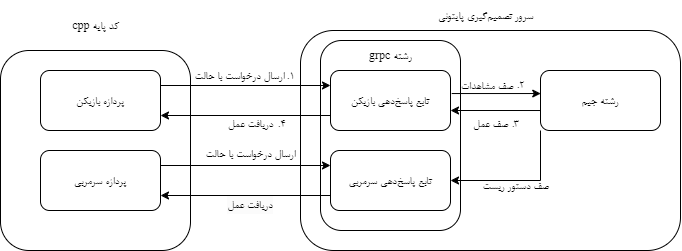
\includegraphics[width=1\textwidth]{images/grpc_gym.png}
    \caption{نحوه کلی ارتباط کد پایه، تصمیم‌گیرنده جی‌آر‌پی‌سی و جیم}\label{fig:gym_grpc}
\end{figure}
در شکل \ref{fig:gym_timing}
به طور دقیق می‌توان ترتیب فراخوانی توابع، و نحوه استفاده از محیط جیم را مشاهده کرد.
کد اجرا کننده \LTRfootnote{Driver Code}
دقیقا فرم مشابه سایر محیط‌های جیم را دارد و از این رابط به طور کامل طبعیت می‌کند.
بخش‌های قرمز رنگ به معنی قفل بودن رشته‌ی اجرایی و در انتظار ماندن برای محتویات صف است.
\begin{figure}[H]
    \centering
    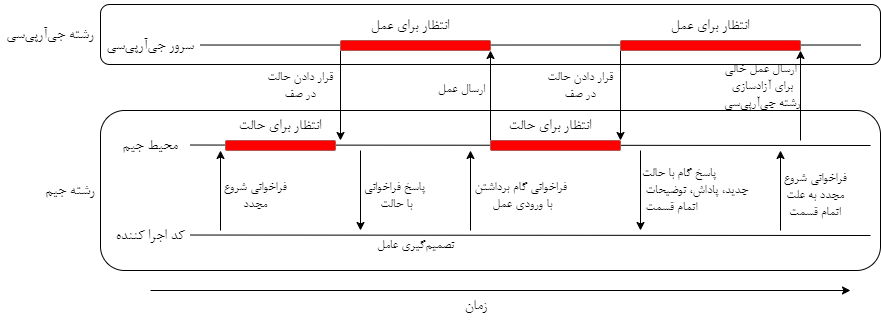
\includegraphics[width=1\textwidth]{images/timing.drawio.png}
    \caption{ترتیب فراخوانی توابع برای اجرای جیم با سرور ربوکاپ}\label{fig:gym_timing}
\end{figure}

داخل شکل، یک قسمت که فقط یک گام تصمیم‌گیری دارد را می‌توان دید. در واقعیت مراحل ((گام برداشتن))
تا قبل از ((فراخوانی شروع مجدد))
به تعداد گام‌های قسمت، تکرار می‌شوند.

برای محیط پنالتی، در صورتی که توپ قابل ضربه‌زدن نباشد، حرکت صحیح همیشه قطع توپ با حداکثر سرعت برای ضربه مجدد است. بنابرین فقط حالت را در شرایطی به جیم ارسال می‌کنیم که توپ قابل ضربه‌زدن باشد.
\subsection{فضای حالت و فضای عمل عامل}
\subsubsection{فضای حالت}
فضای حالت انتخاب‌شده یک بسته ۹ بعدی است، که شامل ویژگی‌های زیر می‌باشد: موقعیت قطبی بازیکن نسبت به مرکز دروازه (اندازه و زاویه)،
موقعیت دکارتی توپ‌ (ایکس و ایگرگ)،
موقعیت دکارتی دروازه‌بان (ایکس و ایگرگ)،
زاویه نسبی حریف نسبت به توپ،
موقعیت قطبی دروازه‌بان نسبت به بازیکن (اندازه و زاویه).

علت اهمیت عاملی مثل زاویه بدن دروازه‌بان، قابلیت حرکت سریع‌تر بازیکنان در راستای مستقیم است. می‌توان عواملی هم‌چون سرعت بازیکنان را نیز اثر داد،
اما برای همگرایی بهتر و سریع‌تر از این عوامل صرف نظر شده.
\subsubsection{فضای عمل}
همان‌طور که گفته‌شد، عامل به صورت خودکار به دنبال توپ می‌رود و ما با کمک یادگیری تقویتی قرار است این عامل را به یادگیری ضربه‌زدن به دروازه برسانیم.
برای این منظور، از رفتار سطح متوسط ضربه با سرعت دلخواه در راستای دلخواه (\lr{KickOneStep})
 استفاده می‌کنیم تا محاسبات مستقل از سرعت توپ قبلی و شتاب توپ شوند.

 به این منظور، فضای عمل ما نیاز است سرعت و زاویه ضربه را تعیین کند.
 با توجه به اینکه برخی الگوریتم‌ها مانند \lr{DQN} بهترین عمل را از بین اعمال ممکن انتخاب می‌کنند و نیاز به فضای عمل گسسته دارند،
و سایر الگوریتم‌ها مانند \lr{DDPG} نیاز به فضای عمل پیوسته دارند،
محیط را در دو حالت گسسته و پیوسته پیاده‌سازی کردیم.

در فضای پیوسته، دو مقدار سرعت توپ و زاویه ضربه به عامل داده می‌شود.
سرعت توپ بین صفر تا یک می‌باشد که نشان‌دهنده سرعت توپ نسبت به حداکثر سرعت ممکن است.
زاویه ضربه بین منفی یک تا یک می‌باشد که نرمال‌شده زاویه مطلق ضربه بین \lr{-۱۸۰} تا ۱۸۰ درجه است.

در حالت گسسته نیز، خروجی ما سرعت توپ و زاویه‌است، اما به‌جای مقادیر پیوسته، زوایای ضربه ممکن را به ۱۲ قسمت مساوی تقسیم کرده‌ایم و سرعت توپ را به ۱۰ قسمت مساوی تقسیم کرده‌ایم.
می‌توان این تقسیم‌بندی را به راحتی تغییر داد و تاثیرات آن روی سرعت یادگیری و نتیجه نهایی آن را بررسی کرد.
در شکل \ref{fig:discretization} می‌توان یک نمونه از تقسیم‌بندی فضای عمل را مشاهده کرد.
از آنجا که سرعت به ۲ درجه تقسیم شده‌است، حالت‌های ممکن آن معادل با نصف حداکثر سرعت توپ و حداکثر سرعت توپ می‌باشد.
\begin{figure}[H]
    \centering
    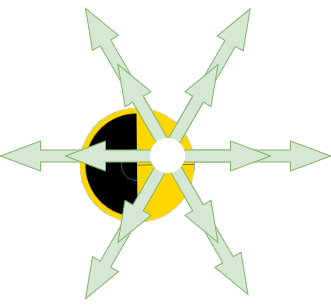
\includegraphics[width=0.45\textwidth]{images/discretization.drawio.png}
    \caption{تقسیم‌بندی فضای عمل به ۶ زاویه و ۲ سرعت}\label{fig:discretization}
\end{figure}
\subsection{طراحی پاداش}
همان‌طور که گفته شد، محیط جیم در حالت‌هایی که توپ قابل ضربه‌زدن است، یا توپ به بیرون رفته و یا توسط دروازه‌بان گرفته‌شده اجرا می‌شود.
در این حالت‌ها باید بر اساس شرایط قبلی، عمل و شرایط جدید پاداشی محاسبه کنیم که به عامل کمک می‌کند تا راحت‌تر به هدف خود نزدیک شود.
\subsubsection{پاداش‌های پایانی}
همانطور که گفته‌شد، چهار حالت پایانی داریم:
\begin{enumerate}
    \item حالت گل زدن: با توجه به رسیدن به هدف، پاداش بزرگی به عامل می‌دهیم که این مقدار، ۱۵۰۰ فرض شده‌است.
    \item حالت بیرون رفتن توپ: از آن‌جا که تنها با ضربات بد این سناریو رخ می‌دهد، پاداش بسیار بزرگ منفی \lr{-۵۰۰} دارد.
    \item گرفتن توپ توسط دروازه‌بان: این حالت از آنجا که بهتر از بیرون رفتن توپ است، پاداش منفی کوچک‌تری دارد و مقدار \lr{-۲۰۰} دارد.
    \item حالت اتمام زمان: به این حالت، پاداش \lr{-۱۵۰} تخصیص داده‌شده، تا عامل در حالتی که هنوز به گل‌زدن نرسیده‌است، مستقیما توپ را به دروازه‌بان ندهد. در واقع با کوچک‌تر در نظر گرفتن این پاداش، عامل را به کاوش بیشتر وا‌می‌داریم.
\end{enumerate}
\subsubsection{پاداش در حالت عادی}
در حالت بین دو ضربه، پاداش را بر اساس سه فاکتور حساب می‌کنیم:
\begin{itemize}
    \item می‌خواهیم عامل را به حرکت به سوی دروازه واداریم، پس از تفاضل فاصله توپ با دروازه در حالت جدید و حالت قبلی به عنوان معیار اصلی استفاده می‌کنیم. در واقع از عکس این فاکتور استفاده می‌کنیم، چرا که کاهش فاصله ویژگی مثبتی است.
    \item نزدیک شدن زیادی به دروازه‌بان ویژگی خوبی نیست، پس از ضریبی از تفاضل فاصله توپ با دروازه‌بان در بین دو حالت استفاده می‌کنیم.
    \item پاداش ثابت \lr{-۱۰} که برای تشویق عامل برای سریع‌تر رسیدن به حالت گل می‌باشد. از این رو که عامل این پاداش را فقط در لحظات ضربه زدن می‌بیند، این فاکتور عامل را به زدن ضربات با قدرت بیشتر تشویق می‌کند.
\end{itemize}
\section{پیاده‌سازی یادگیری تقویتی}
\subsection{پیاده‌سازی شبکه کیو عمیق}
با کمک کتاب‌خانه \lr{PyTorch}،
یک شبکه عصبی با یک لایه پنهان و تابع فعال‌سازی \lr{ReLU} پیاده‌سازی شد.
این شبکه، ورودی به ابعاد فضای حالت محیط دارد و خروجی به اندازه فضای عمل است.
تمامی ابرپارامتر‌های ما به عنوان ورودی تابع سازنده مدل داده می‌شوند.

سپس تابع یادگیری فراخوانی می‌شود، که ورودی آن مشخص می‌کند که چند گام از محیط برای آموزش استفاده شود.
این تابع، با استفاده از الگوریتم \lr{DQN}،
به تعداد مراتب در محیط گام بر می‌دارد و تجارب را به بافر اضافه می‌کند. در گام‌هایی که شماره آن ضریبی از ابرپارامتر \lr{update\_freq} است،
شبکه را به کمک گزینش ریزدسته‌ای از تجربیات و الگوریتم گرادیان، به‌روز می‌کند.
همچنین در گام‌هایی که شماره آن ضریبی از ابرپارامتر \lr{target\_update\_freq} است،
شبکه هدف را به‌روز می‌کند.

همانطور که در فصل‌های قبل اشاره شد، نرخ کاوش تصادفی به مرور زمان کاهش می‌یابد.
در ابرپارامتر‌ها، نرخ اولیه، نرخ نهایی، و درصد گام‌هایی که این کاهش نرخ در آن رخ می‌دهد با 
پارامتر‌های \lr{epsilon\_start}، \lr{epsilon\_end} و \lr{epsilon\_fraction} مشخص می‌شود.
پارامتر \lr{epsilon\_fraction} در واقع نشان می‌دهد که در چند درصد اول گام‌های آموزشی، نرخ کاوش تصادفی به نرخ نهایی می‌رسد.
در شکل \ref{fig:epsilon_decay} می‌توان نمودار کاهش نرخ کاوش تصادفی را مشاهده کرد.
در این مثال آموزش برای ۱۰۰۰ گام رخ داده، نرخ اولیه ۱ و نرخ نهایی ۰.۵ انتخاب شده‌است، و کسر اپسیلون
\LTRfootnote{Epsilon fraction}
 ۰.۱ است.
\begin{figure}[H]
    \centering
    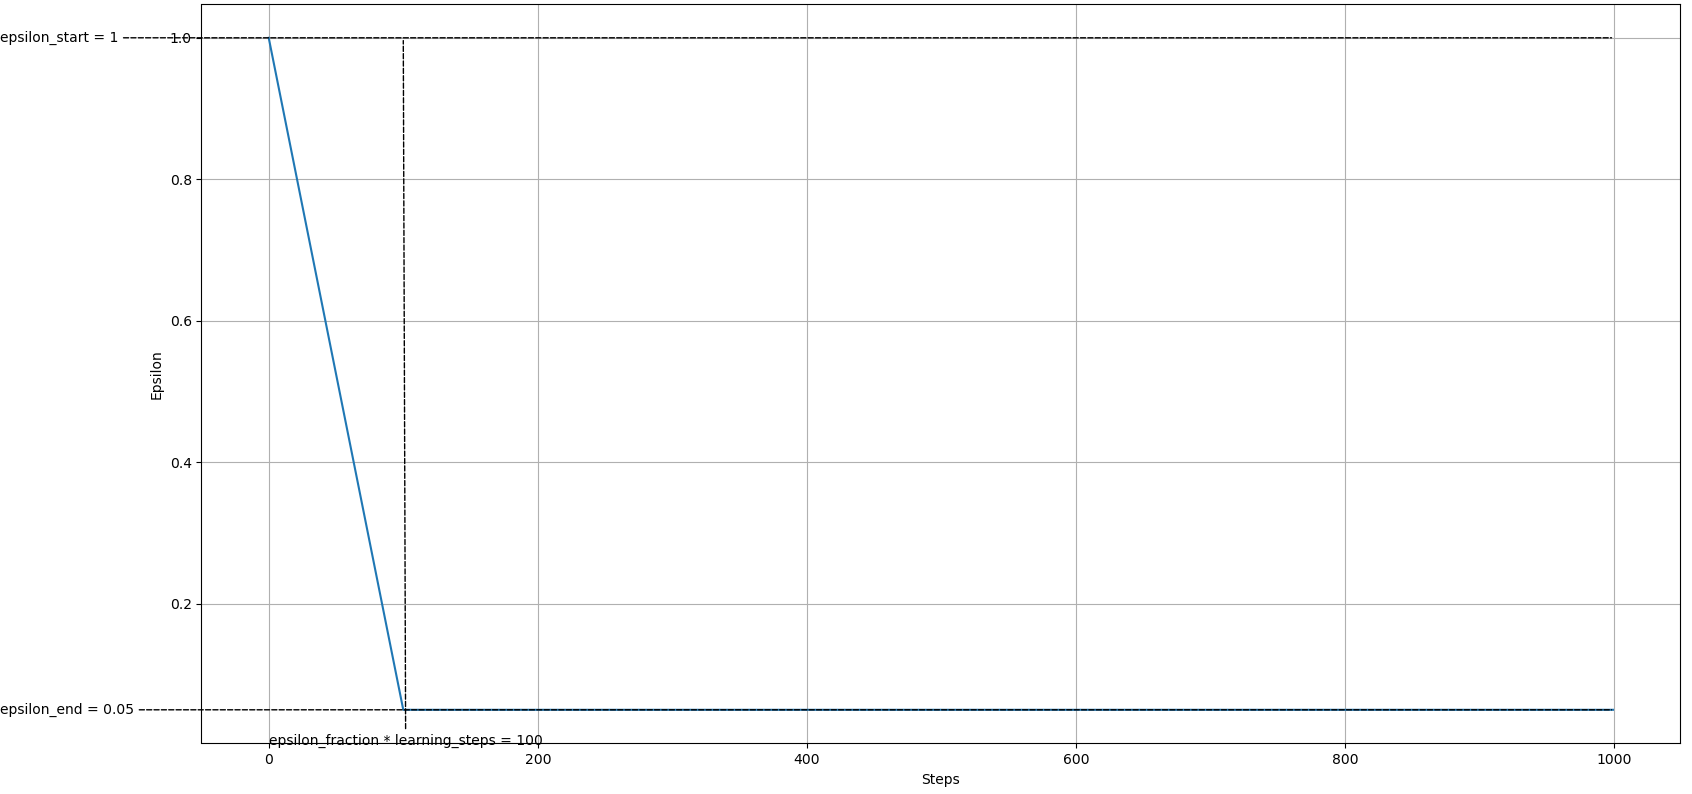
\includegraphics[width=1.1\textwidth]{images/epsilon_decay_2.png}
    \caption{کاهش نرخ کاوش تصادفی در طی آموزش}\label{fig:epsilon_decay}
\end{figure}
\subsection{پیاده‌سازی سایر الگوریتم‌ها به کمک کتابخانه}
یکی از مهم‌ترین مزایای پیاده‌سازی رابط استاندارد جیم، ایجاد امکان استفاده از پیاده‌سازی‌ها و کتاب‌خانه‌های از‌پیش‌موجودی اند که وجود دارند.
با توجه به اینکه اکثر الگوریتم‌های یادگیری تقویتی در کتاب‌خانه‌هایی مانند \lr{Stable Baselines} و \lr{OpenAI Baselines} پیاده‌سازی شده‌اند،
می‌توان از این کتاب‌خانه‌ها برای آموزش عامل‌ها استفاده کرد.
در این پروژه، از کتاب‌خانه \lr{Stable Baselines} برای آموزش عامل‌ها استفاده شده‌است.
کافی‌ست ابتدا یک محیط جدید از جیم تعریف کنیم، مدلی از الگوریتم دلخواه بسازیم، و سپس با استفاده از تابع \lr{learn}
مدل را به تعداد گام‌های دلخواه آموزش دهیم.
\begin{figure}[H]
    \centering
    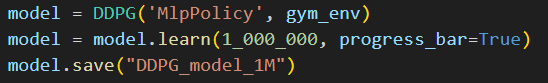
\includegraphics[width=0.75\textwidth]{images/sb3.png}
    \caption{استفاده از کتاب‌خانه \lr{Stable Baselines 3}}\label{fig:sb3}
\end{figure}
طبق مستندات این کتاب‌خانه، می‌توان به مدل توابعی را به عنوان ورودی داد تا در حین آموزش به صورت مکرر و پس از تعداد گام دلخواه به صورت تناوبی صدا زده‌شوند.
 از این توابع می‌توان برای ارزیابی مدل به صورت تناوبی، و ذخیره‌سازی در حین آموزش استفاده کرد که برای مقایسات فصل بعدی بسیار کاربردی است.
\section{جمع‌بندی}
در این فصل، مروری بر راه‌های مختلفی که می‌توان از آن‌ها برای پیاده‌سازی یادگیری تقویتی استفاده کرد، داشتیم.
از جمله این روش‌ها، استفاده از \lr{HFO} و \lr{Pyrus} بودند.
سپس با معرفی پلتفرم جیم، نحوه پیاده‌سازی محیط‌های جدید و تعریف فضای حالت و عمل را مورد بررسی قرار دادیم.

در ادامه، نحوه ادغام این محیط‌ها با فضای ربوکاپ و پیاده‌سازی یک محیط جدید به نام پنالتی را مورد بررسی قرار دادیم.
سپس نحوه پیاده‌سازی یک عامل یادگیری تقویتی با استفاده از شبکه کیو عمیق و کتاب‌خانه \lr{Stable Baselines} را بررسی کردیم.
در فصل بعدی، نتایج این پیاده‌سازی‌ها را مورد بررسی قرار می‌دهیم.